\chapter{典型应用观测与画像分析}\label{chap:profiling}

\section{概述}

% 吵闹邻居

指定混部方案涉及到对于典型应用的选取与应用画像分析。其中对于典型应用的选取需要符合当前数据中心的需求,同时需要涉及足够多的领域,这样才能够充分挖掘混部可能。随后则需要依据混部目标的部署方案,来决定可观测性系统的搭建方案,同时需要从不同的维度来对应用的运行状况进行细致全面的指标采集,这样得到的指标数据才能更具分析价值。完成上述准备之后,还需要设计一系列实验来对应用进行探测,结合相关研究,本文分别在有无干扰的设置下对应用性能进行探测,在干扰的选择上,以常用的CPU、Cache、Memory、IO、Network干扰作为测度选项。

\section{云场景典型应用选择}

% 介绍每个应用

本文研究结合了在云厂商中的实践经验,选择了如表~\ref{tab:typical_application}所示的如下10个应用作为数据中心的典型应用进行分析。应用涵盖了传统数据库、键值存储、消息中间件、大数据、媒体处理等领域。跨领域地选择应用主要考虑到不同专业领域应用的运行模式差异较大,因此就更有可能在硬件资源的使用方面更加差异化,其中数据库类型的应用,由于数据保存在磁盘上,因此在进行大量数据查询时,对于IO资源的需求较高,键值存储类应用依赖对于内存读写来完成数据操作,因而对于内存资源的需求较高,网络服务类型应用通常都是交互式的,因此对延迟十分敏感,也意味着需要更快地的分配时间片,媒体处理应用则会大量地使用到CPU上的编解码单元,因此对时间片数量的需求更高,这些在资源使用上的差异化为混部提供了可能。

\begin{table}
    \bicaption{\quad 典型应用选择}{\quad Typical application selection}% caption
    \label{tab:typical_application}
    \footnotesize% fontsize
    \setlength{\tabcolsep}{4pt}% column separation
    \renewcommand{\arraystretch}{1.5}% row space 
    \centering
    \begin{tabular}{lc}
        \hline
        %\multicolumn{num_of_cols_to_merge}{alignment}{contents} \\
        %\cline{i-j}% partial hline from column i to column j
        类型 & 应用\\
        \hline
        SQL & mysql、clickhouse\\
        NoSQL & elasticsearch\\
        Web Server & nginx\\
        K-V Store & redis、keydb、memcached\\
        Message Queue & kafka\\
        Big Data & hibench\\
        Media & render\\
        \hline
    \end{tabular}
\end{table}

\section{在线指标采集系统}

% 按维度解释每个指标的含义

本研究构建在线指标采集系统基于两个目标,首先在可观测性上,围绕虚拟机、应用监控,构造多维度的指标采集系统,其次还需要实现对于上述选取应用的QoS监控,一方面QoS数据能够与其他性能指标一同纳入分析体系,共同参与典型应用的画像过程,另一方面实时的QoS监控也是本研究中应用性能劣化监测的手段之一,能够为后续调度提供劣化信息并作为不同调度算法的评价指标。

在线指标采集系统将定义每台服务器为一个监控节点,如图~\ref{fig:montor_arch}所示,每个节点依据承担负载及监控关系划分为master与node两种角色,一个节点可同时兼任两种角色。其中node节点负载承担云应用负载,实验中一般部署Server应用,同时node作为被监控的对象,需要提供指标监控服务,考虑到监控服务实质也是应用,因而需要一定的隔离措施来避免采集过程中产生的噪声。master 一般不承担应用负载,实验中一般部署Client应用,同时作为监控者,需要提供数据采集、存储和查询服务,并按照预定义的配置不断从 node 的监控服务中采集指标,同时也提展示、分析等额外功能。

\begin{figure}[!htbp]
    \centering
    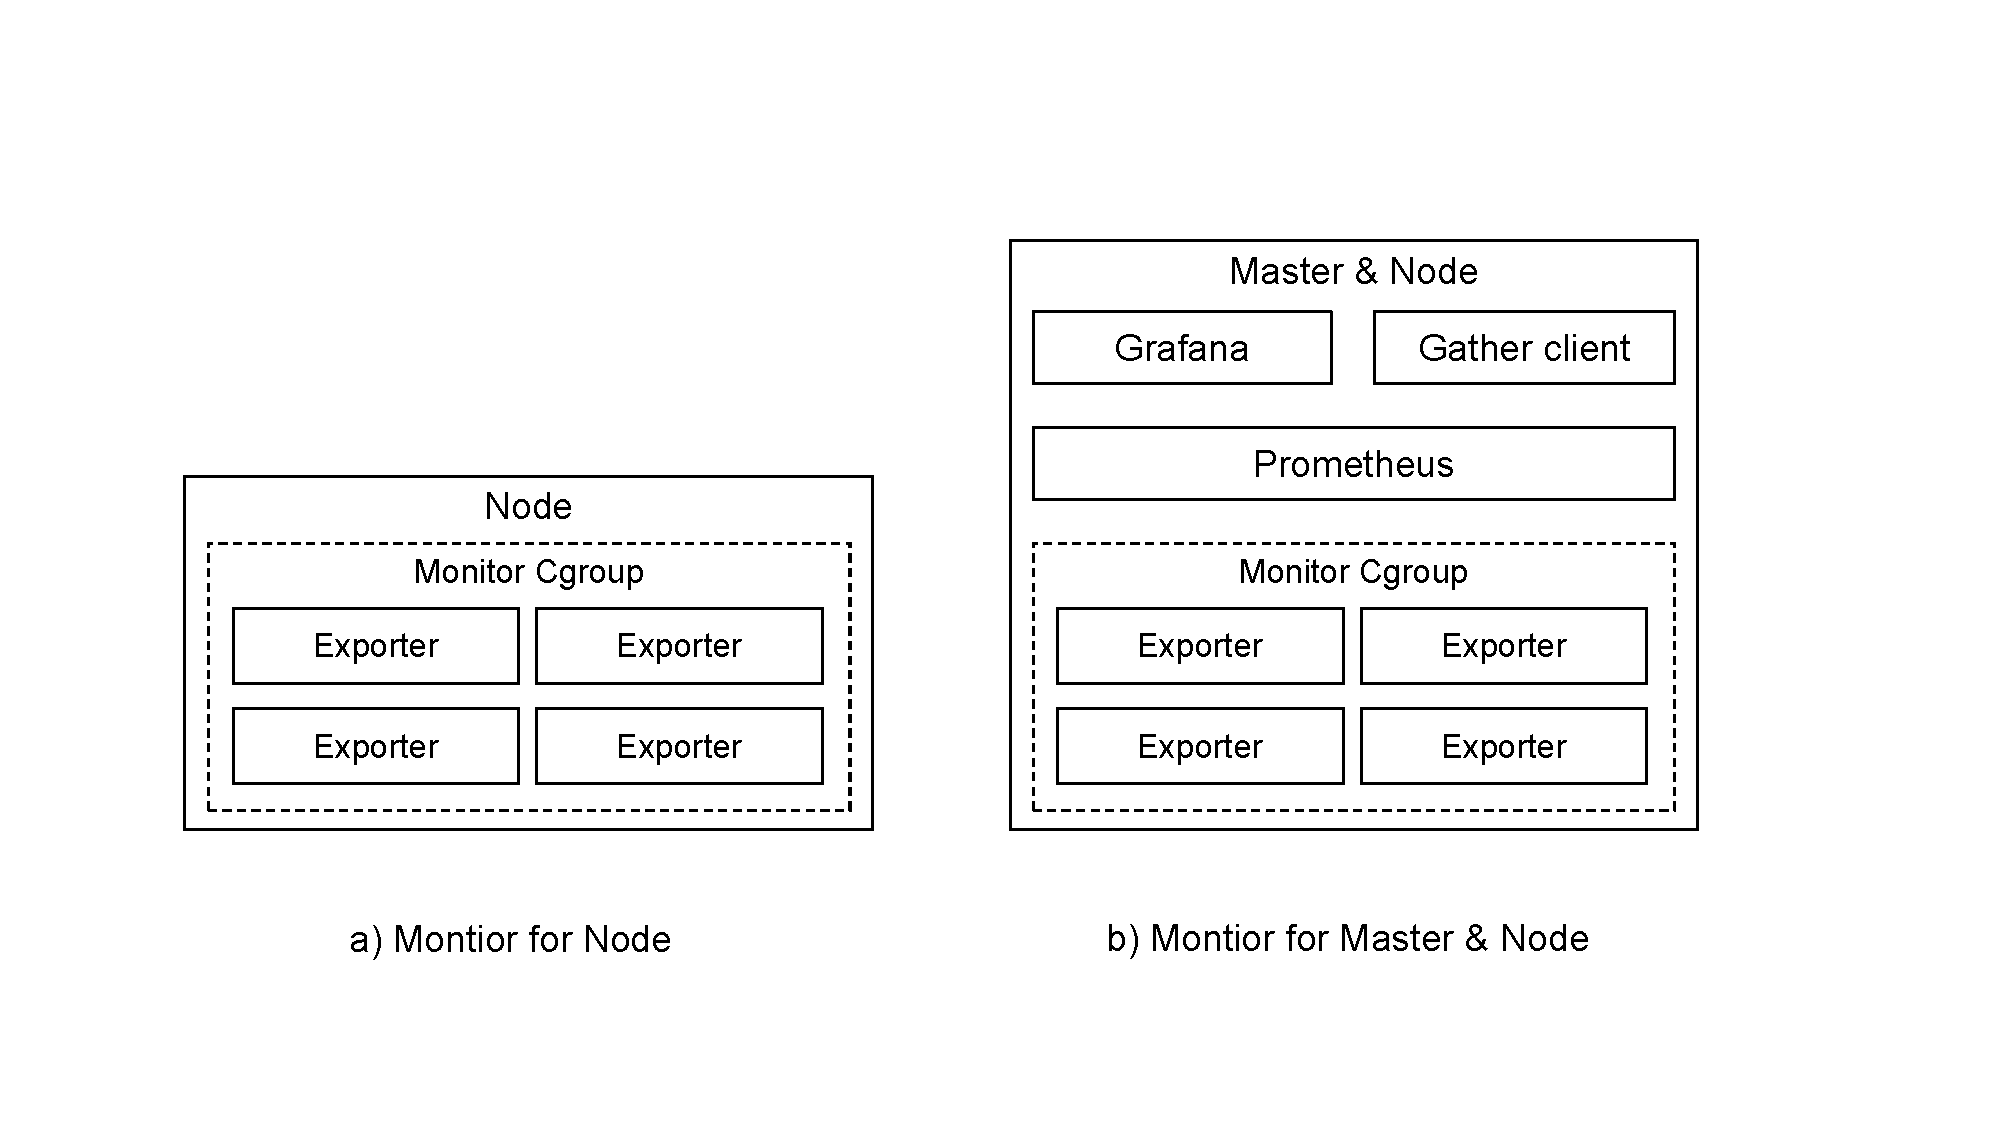
\includegraphics[width=1.0\textwidth]{montor_arch}
    \bicaption{\quad 监控系统中不同角色的区别}{\quad The differences between different roles in the monitoring system}
    \label{fig:montor_arch}
\end{figure}

指标监控框架实现中考虑实时性与灵活性,因而采用主动轮询、被动采集的模式,选择基于Prometheus生态进行具体实现。不同的监控节点角色决定了部署在其中监控组件的不同。node 节点需要安装一系列Exporter组件来提供各层级的指标监控服务,并提供容器化依赖Cgroup来实现与业务域的隔离。master节点则需要安装Prometheus Server、Grafana等组件,通过预定义的服务发现配置、指标聚合策略及采集设置等,完成采集、存储与展示工作。

实现多维度指标采集核心在于Exporter的设计,如图所示,本研究中从Host、Hypervisor、App三个维度设计了6种不同的Exporter,总采集指标数量如表~\ref{tab:metric_list}所示,达到344个,涉及到CPU、Cache、Memroy、IO、Network等子系统。

\begin{figure}[!htbp]
    \centering
    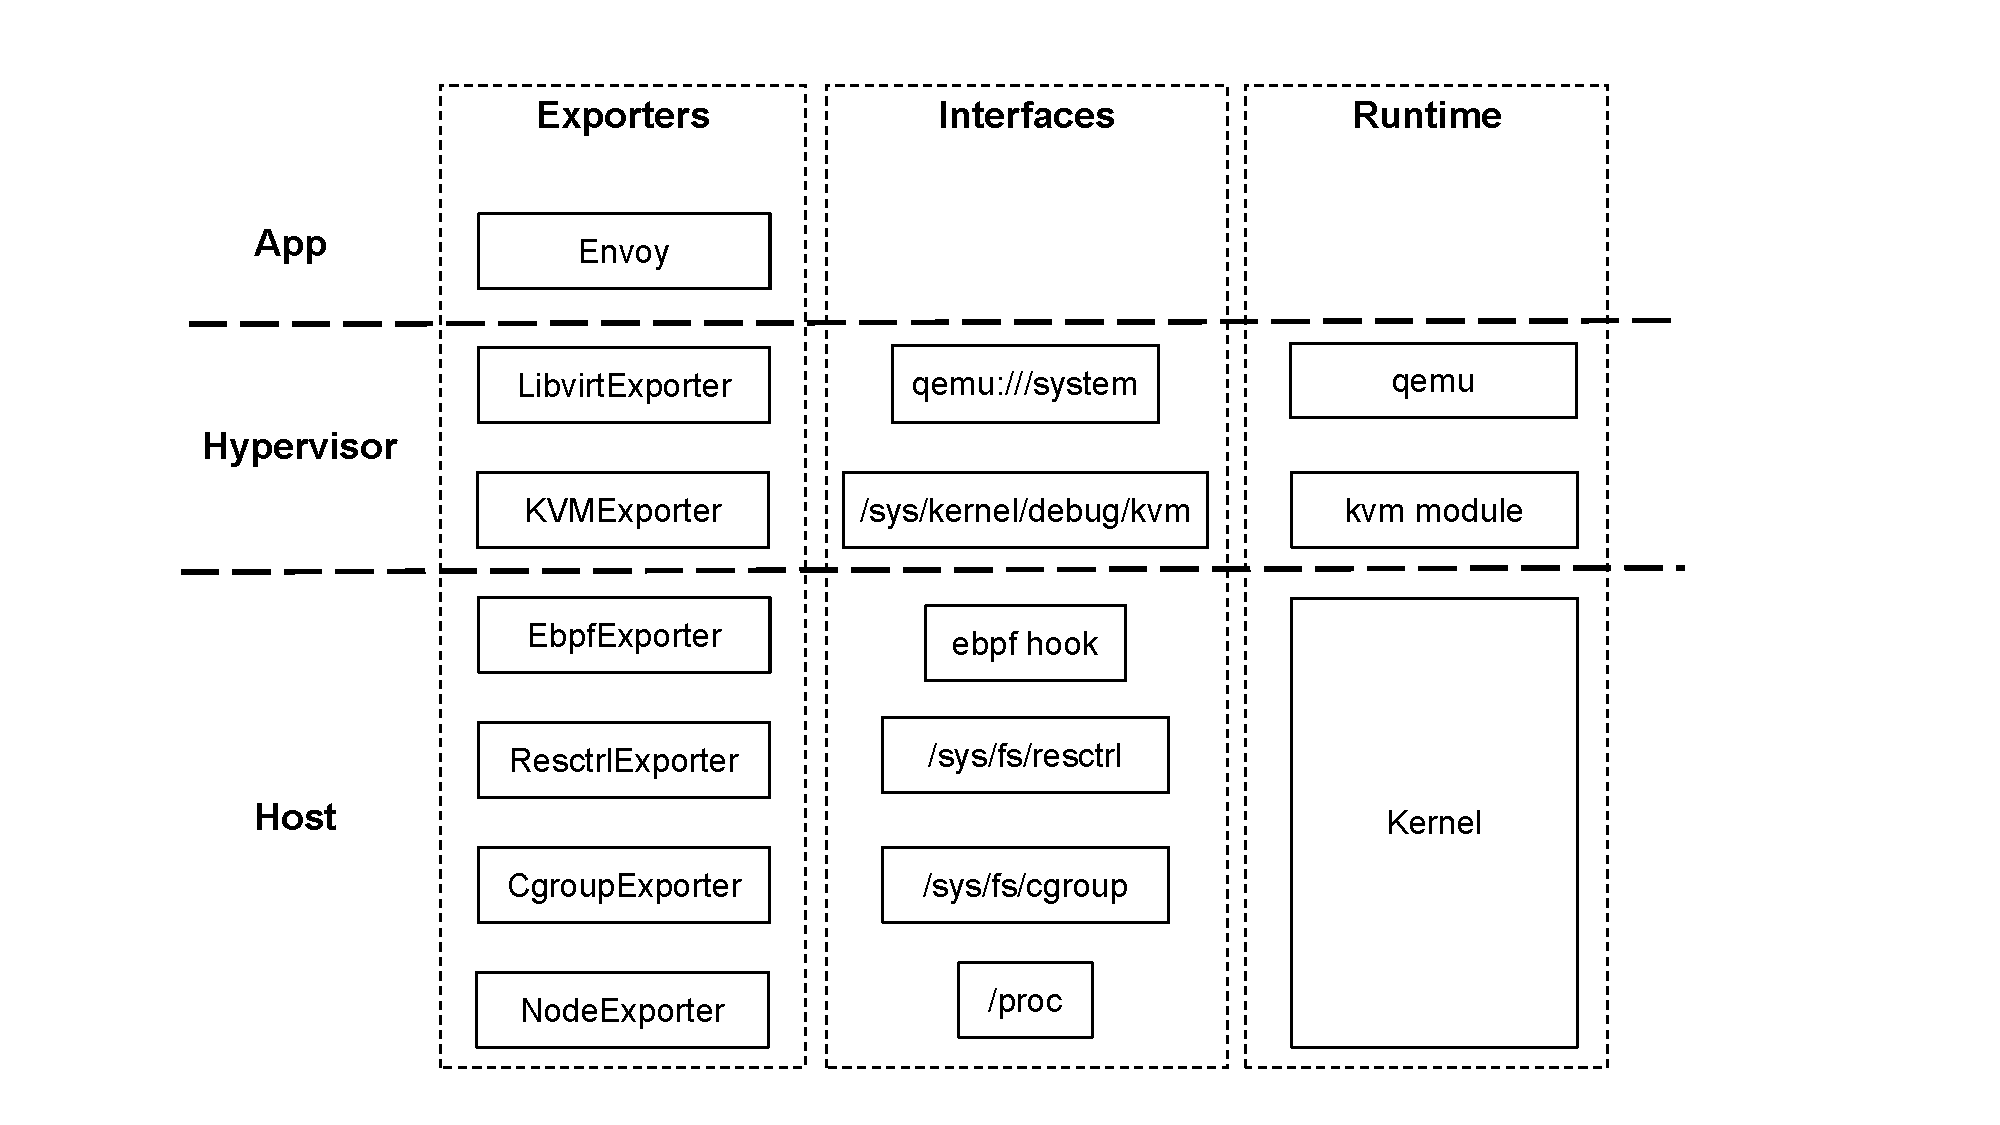
\includegraphics[width=1.0\textwidth]{exportes}
    \bicaption{\quad Exporters设计}{\quad Exporters Design}
    \label{fig:exportes}
\end{figure}

LibvirtExporter 使用Libvirt API采集数据,获取虚拟机 vCPU、Memory、Network、Block IO 等虚拟资源的使用情况。KVMExporter 读取KVM Kernel Debug fs 获取更详细的虚拟机运行时指标,这些指标通常是KVM相关模块中的事件计数,如 vm exit、io exit 等,能够反映出vCPU的工作状态。

NodeExporter 则通过读取 Kernel 提供 的用户交互接口,获取CPU、网络、存储等各个子系统的详细信息,获取Host主机上的总体资源使用情况。ResctrlExporter则通过 Intel RDT 技术,获取更细粒度的性能指标,如L3 Cache容量,Memory Bandwidth,默认情况下,ResctrlExporter会对系统全局进行监控,当用户创建了 Monitor Group 之后,则会将其添加到监控目标中,实验中通过vm info map构建Monitor Group 以对虚拟机进行监控。

EbpfExporter 启动之后会加载编译好的ebpf代码,并将采集到的数据和转化为Metric来对外部提供监控服务。进程在使用Host资源特别是硬件资源时,通常会涉及到多条资源分配的关键路径,通过Ebpf能够在这些关键路径上进行插桩,从而反映进程使用这些资源的频率及耗时信息。如图~\ref{fig:syscall_hook}所示,当前实现了对进程系统调用的相关信息统计,通过在系统调用进入与退出的位置插入ebpf代码,以Cgroup为粒度统计每个系统调用的频率和总时长。

\begin{figure}[!htbp]
    \centering
    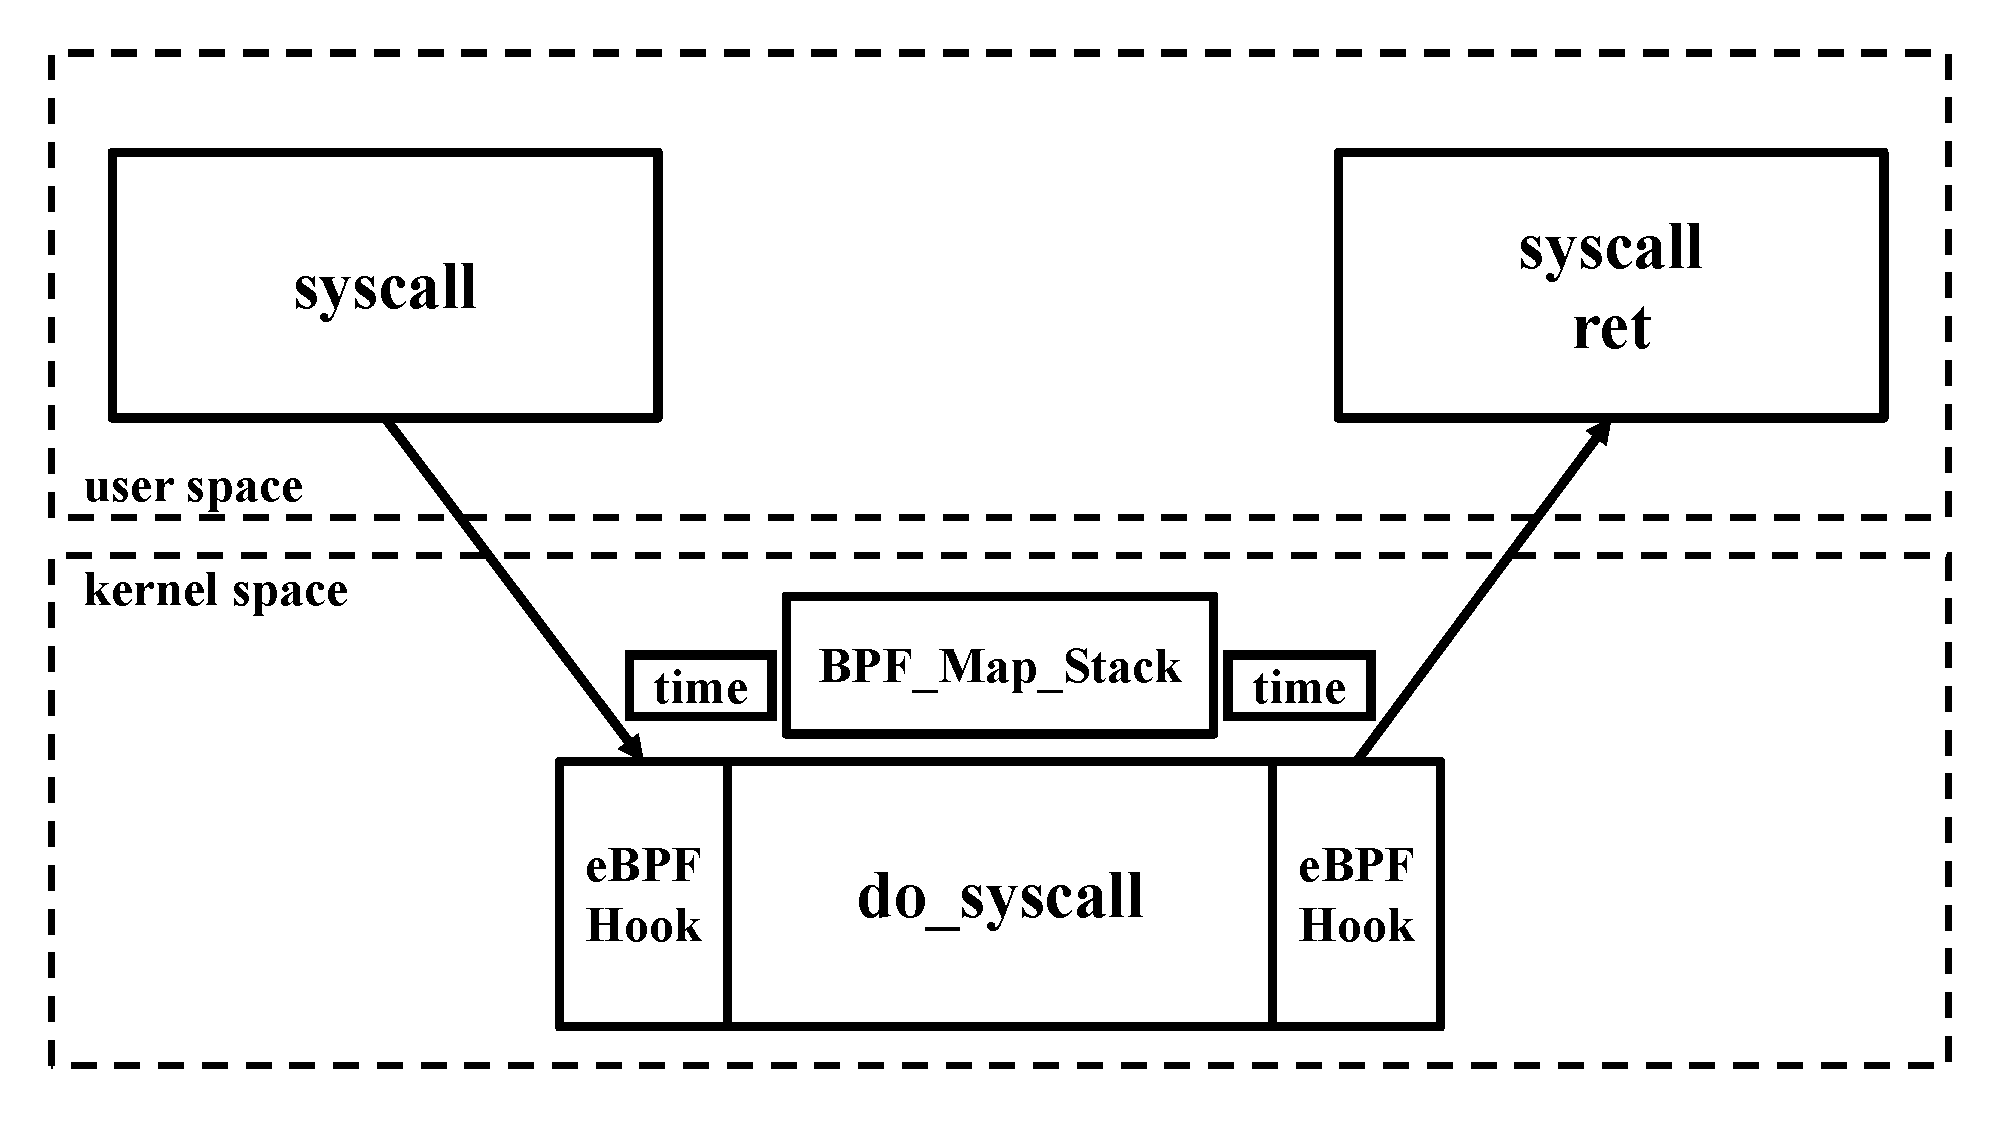
\includegraphics[width=1.0\textwidth]{syscall_hook}
    \bicaption{\quad eBPF Syscall插桩}{\quad eBPF Syscall Hooking}
    \label{fig:syscall_hook}
\end{figure}

对于常规进程而言,其对系统资源的使用一般依赖系统调用作为统一入口,因此在此入口处的插桩能够对相关数据进行抓取。然而虚拟机是一种特殊的进程,尽管其对于资源的使用也最终都会由Host上的对应设备来完成模拟,但不同之处在于,虚拟机在开启硬件加速之后,部分资源的使用会直接在内核态处理,这样虽然保证了虚拟机的性能,但也同时也增加了插桩的复杂度。现阶段提供的系统调用入口处的插桩能够监测Qemu程序在用户态下请求使用Host资源的情况,如图~\ref{fig:vhost_net}所示,当前主要考虑到Qemu进程中仍有线程主要在用户态执行,这些指标能够对其资源使用情况进行监控。

\begin{figure}[!htbp]
    \centering
    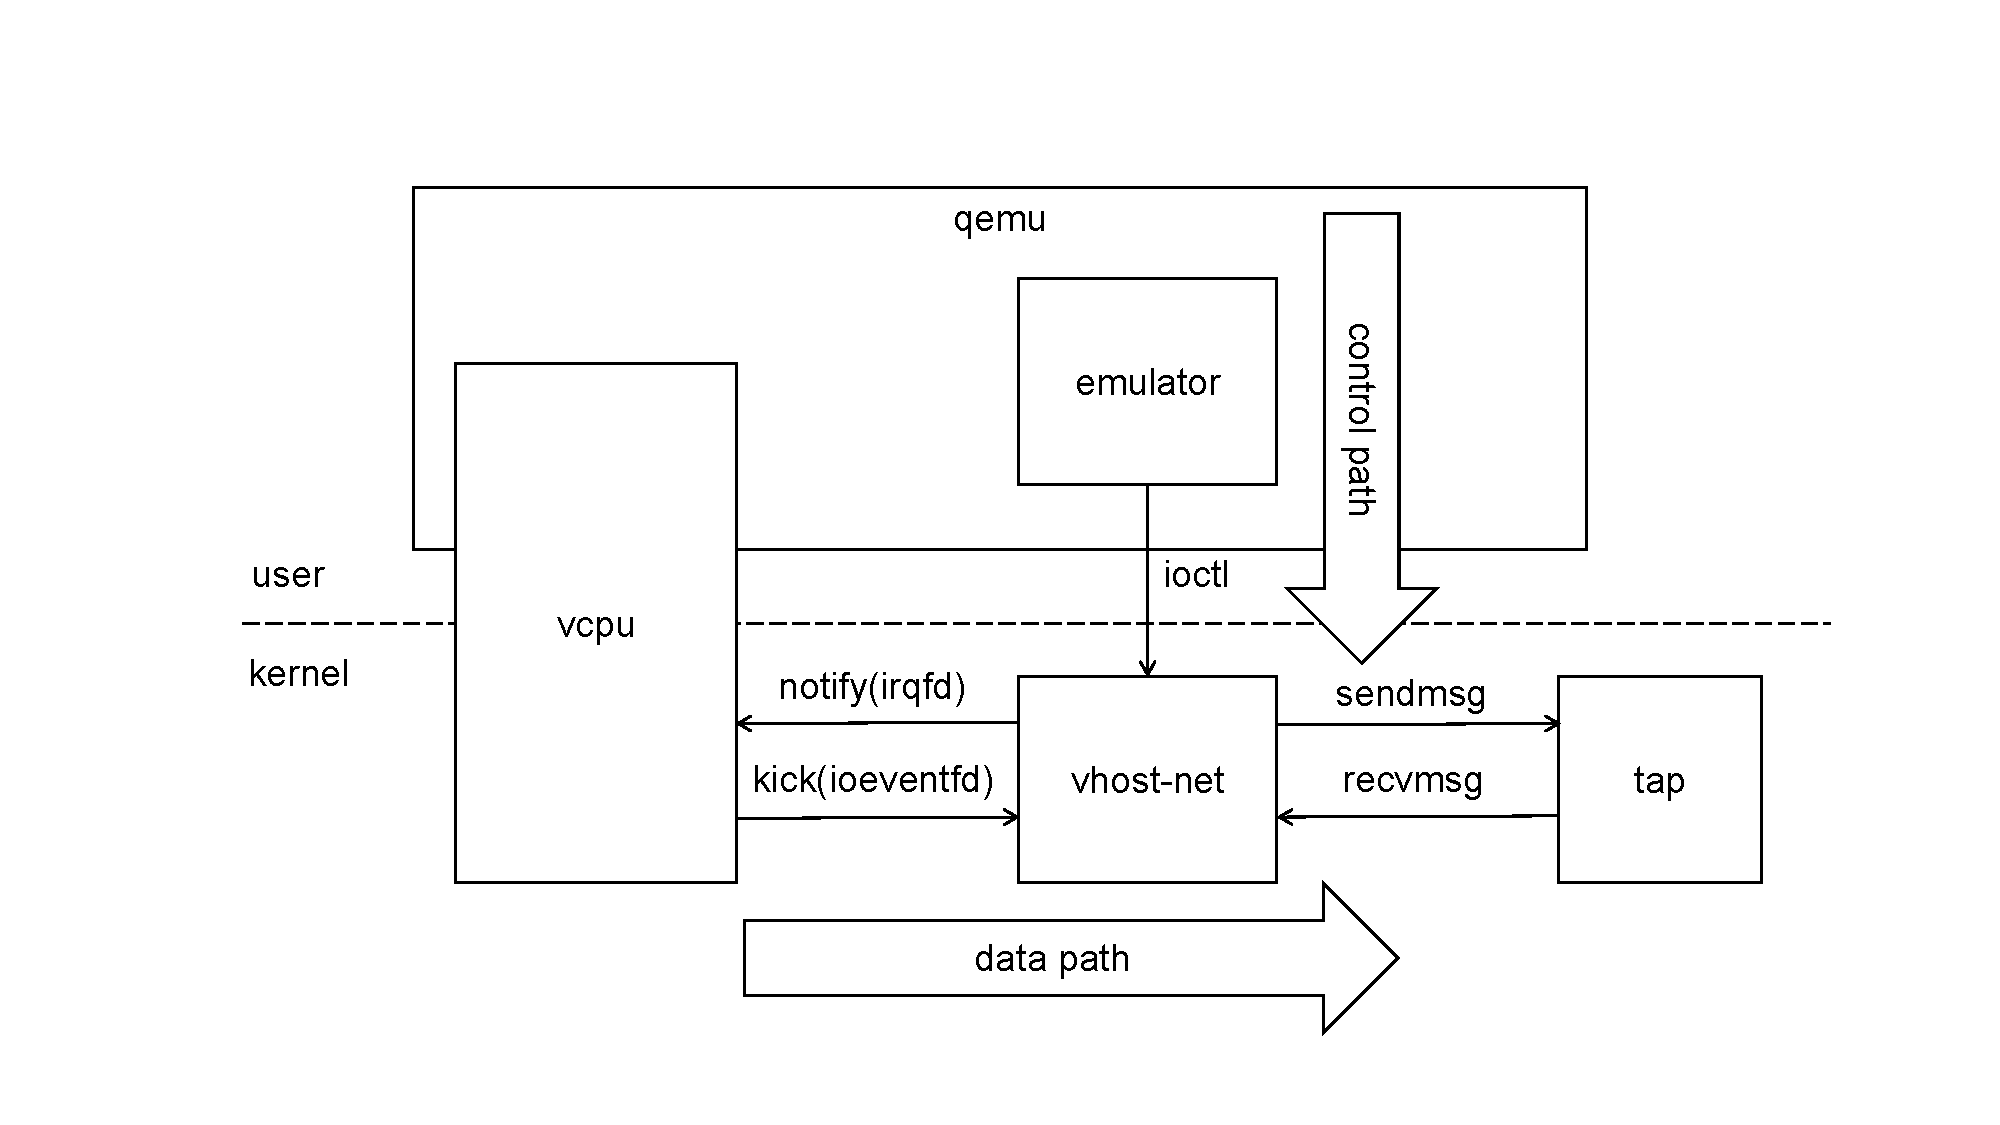
\includegraphics[width=1.0\textwidth]{vhost_net}
    \bicaption{\quad Qemu vHost 网络}{\quad Qemu vHost Net}
    \label{fig:vhost_net}
\end{figure}

Prometheus中积累的指标数据通常需要经过初步的聚合才具有分析价值,如对于某一个计量值,其在单位事件内的变化速率相较于瞬时值来说更有统计价值,当前实验配置中会以4s为窗口进行聚合,聚合规则同样以配置呈现,即可用于Grafana中进行实时监控信息展示,也可以在Gather API 中使用以将数据进行批量导出。

\begin{table}
    \bicaption{\quad 指标列表}{\quad Metric list}% caption
    \label{tab:metric_list}
    \footnotesize% fontsize
    \setlength{\tabcolsep}{4pt}% column separation
    \renewcommand{\arraystretch}{1.5}% row space 
    \centering
    \begin{tabular}{lcc}
        \hline
        %\multicolumn{num_of_cols_to_merge}{alignment}{contents} \\
        %\cline{i-j}% partial hline from column i to column j
        层级 & 来源 & 指标\\
        \hline
        Host & Kernel(271) & [cpu] sys_time、user_time、freq ... \\
        & & [mem] usage、avail、swapfree、bounce、hugepage ...\\
        & & [network] transmit、netstat、sockstat、ip、speed ...\\
        & & [disk]flush requests、flush request time、read、write ...\\
        & & ...\\
        & eBPF(2) & [syscall] count、duration\\
        & Resctrl(3) & llc cap、mem b/w local、mem b/w total\\
        Hypervisor & Libvirt(68) & [vcpu] sys_time、user_time、wait、delay...\\
        & & [mem] usable、avail、dick cache、rss ...\\
        & & [perf] cycle、instruction、cache miss ...\\
        & & [block] flush request、flush time、read、write ...\\
        & & [interface] receive、transmit ...\\
        & & ...\\
        & KVM(59) & vm_exit、io_exit、irq_exit、irq_inject、halt_poll ...\\
        App & Log/Envoy & qos, latency, rate, score ...\\
        \hline
    \end{tabular}
\end{table}

\section{干扰实验设计}

% 干扰的选择,干扰有效性及噪声控制

在干扰应用的选择上,选择使用stress-ng来模拟产生不同类型的资源干扰。stress-ng是Linux系统中常用的压力测试工具,能够通过模拟各种负载来检测系统的稳定性和性能,实验中利用其模拟各种压力负载的特性来分别从CPU、内存、I/O、Cache、Network上制造干扰,观测应用在不同干扰下的劣化情况。stress-ng拥有诸多可调整的参数选项,用于定制化不同的压力场景,本课题选用如表~\ref{arg_list}所示参数制造上述类型的干扰。对于AVX干扰应用通过开发程序实现,根据传入的参数,循环执行AVX2/AVX512指令来产生不同强度的压力

\begin{table}
    \bicaption{\quad stress\_ng 参数列表}{\quad stress\_ng args list}% caption
    \label{tab:arg_list}
    \footnotesize% fontsize
    \setlength{\tabcolsep}{4pt}% column separation
    \renewcommand{\arraystretch}{1.5}% row space 
    \centering
    \begin{tabular}{lcc}
        \hline
        %\multicolumn{num_of_cols_to_merge}{alignment}{contents} \\
        %\cline{i-j}% partial hline from column i to column j
        子系统 & 参数 & 说明\\
        \hline
        CPU	    & --cpu	& 循环执行sqrt(rand())的线程数量\\
	            & --cpu-load & 线程负载的比率\\
        Cache	& --cache & cache抖动线程数量\\
	    & --cache-level	&测试指定等级的Cache\\
	    & --icache	&指令cache抖动的线程数量\\
        IO	    & --io	&循环执行sync()的线程数量\\
	            & --iomix	&执行混合I/O操作的线程数量\\
	            & --hdd	&循环执行write()/unlink()的线程数量\\
	            & --seek	&执行随机seek I/O的线程数量\\
        Memory	& --vm	&循环执行匿名mmap的线程数量\\
	            & --vm-bytes	&执行vm操作的buffer大小\\
	            & --memrate	&执行read/writes的线程数量\\
	            & --memrate-bytes	&执行内存操作的buffer大小\\
	            & --malloc	&执行malloc/realloc/free的线程数量\\
	            & --memcpy	&执行memory copy的线程数量\\
        Network	& --sock	&执行Socket I/O的线程数量\\
	            & --epoll	&执行epoll处理的线程数量\\
        \hline
    \end{tabular}
\end{table}

% \section{画像分析与结论}

% \subsection{无干扰实验下的应用资源使用倾向分析}

% \subsection{有干扰实验下的应用资源敏感度分析}

% \section{本章小结}

